\documentclass{article}
\usepackage[utf8]{inputenc}
\usepackage{amsmath}
\usepackage{graphicx}
\usepackage{amsthm}
\usepackage{amssymb}

\title{\textbf{Fondamenti di Statistica e Probabilità}}
\author{Pietro Bonardi}
\date{Marzo 2020}
\newtheorem{definition}{Definizione}[section]
\newtheorem{teorema}{Teorema}[section] 
\newtheorem{dimostrazione}{Dimostrazione}


\begin{document}

\maketitle 
\tableofcontents
\newpage

\section{Introduzione}
In questo documento si mostreranno gli aspetti di basi della statistica, in particolare si focalizza sulla descrittiva ed inferenziale. È inteso come un documento per ripassare i concetti principali. 

\section{Statistica Descrittiva}
    \paragraph{Statistica Descrittiva}Per definizione si intende quella raccolta di metodi e strumenti matematici atti ad organizzare una o più serie di dati in modo tale da evidenziarne in forma \textbf{\textit{sintetica}} eventuali:
    \begin{itemize}
        \item Simmetrie
        \item Periodicità
        \item Leggi di altro genere
    \end{itemize}
        Ovvero in grado di descriverne in maniera "intuitiva" informazioni implicite. 
    
    
    \paragraph{Popolazione} L'insieme degli elementi cui si riferisce l'indagine statistica.
     È un insieme limitato costituito da \textit{osservazioni}.
    \paragraph{Caratteri} I dati variano in funzione dei modi di presentarsi.
    \begin{itemize}
        
        \item Caratteri qualitativi, quando sono qualità o dati non numerici.
        \begin{itemize}
            \item Nominali,descrivono una caratteristica, fenomeno, che si manifesta con degli attributi, modalità che non hanno un ordinamento.
            \item Ordinali descrivono una caratteristica, fenomeno, che si manifesta con degli attributi, modalità che hanno un ordinamento naturale.
        \end{itemize}
        \item Caratteri Quantitativi, quando le grandezze sono misurabili e si manifestano con dei numeri o valori.  
        \begin{itemize}
            \item Discreti, quando assumono valori numerabili.
            \item Continui quando assumo valori sull'asse $R$.
        \end{itemize}
        
    \end{itemize}
    

    \subsection{Rappresentazioni numerica di dati statistici}
    Supponiamo di avere: 
     $E= \{ x_1,x_2,...,x_n \}\\$ 
        
    È corretto raggruppare i dati in modalità ed associare a ciascuna di esse il numero di volte che compaiono in $E$. Si definisce quindi l'insieme
    $S=\{s_1,s_2,...,s_N\}$, delle possibili modalità dove "$_N$" è il numero totale di modalità.
    
    
    \begin{definition}{Frequenza Assoluta} 
    Si dice frequenza assoluta della modalità $s_j$ dove 
    $j = 1,...,N$: 
    
    $f_j$ = numero di elementi di $E$ con valore $s_j$
      \end{definition}
    
    \begin{definition}{Distribuzione Frequenza Assoluta} 
    Definita come $$f\colon \{s_1,s_2,...,s_N\}\mapsto f_j$$
    \end{definition}
    
   \begin{definition}{Frequenza Cumulata Assoluta}
    $$ F_j= \sum_{k:s_k \leq s_j} f_k$$
    \end{definition}
    
    \begin{definition}{Frequenza Relativa}
        $$p_j=\frac{f_j}{n}$$ dove $n$ è la grandezza dell'insieme $E=\{x_1,x_2,...,x_n\}$.
    \end{definition}
    
    \begin{definition}{Frequenza Cumulata Relativa}
        $$ P_j= \sum_{k:s_k \leq s_j} p_k$$
    \end{definition}
    
    Quando siamo nel caso \textbf{continuo} oppure in quello discreto ma con molte modalità, è corretto dividere in classi. 
    \begin{definition}{Classe}
        Una classe di una modalità è un sotto insieme di $S$.
        Si partizione quindi la modalità tale che: 
        $\\C_i\cap C_j = \emptyset$  $\forall i,j \\
        C_i\cup C_j =S=\{s_1,s_2,...,s_N\}\\$
        
        
        Alle classi sono associati dei valori: 
        \begin{itemize}
            \item Confine superiore, l'elemento più grande di $C_j$
            \item Confine inferiore, l'elemento più piccolo di $C_j$
            \item Semisomma, $\frac{Superiore + Inferiore}{2}$
        \end{itemize}
    \end{definition}
    \newpage
    \subsection{Indici di tendenza  centrale o di posizione}
    In generale gli indici di posizione o misure di tendenza centrale vengono chiamati medie.
    \begin{definition}{Medie}
    Data una variabile quantitativa $X$, che assume su $N$unità statistiche i valori non decrescenti $x_1, x_2,...,x_N$, sono denominate \textbf{medie} quelle particolari funzioni che soddisfano le seguenti proprietà:  
      \begin{itemize}
        \item \textbf{internalità}, la media non deve essere inferiore al   più piccolo dei valori osservati né superiore al più grande,     ovvero deve essere interna al campo di osservazione
        \item \textbf{moltiplicativa}, la media segue le variazioni         dell’unità di misura
        \item \textbf{monotonicità}, ovvero se almeno uno dei valori         aumenta, o diminuisce, restando invariati tutti gli altri, la     media aumenta, o diminuisce.
        \end{itemize}{}
      \end{definition}
    

    La funzionalità degli \textbf{\textit{Indici di Tendenza Centrale}} è di determinare un solo valore per rappresentare la serie intera di dati, quindi essere in grado di sintetizzare. 
    
    \begin{itemize}
        \item \textbf{Moda}, è calcolabile per ogni tipo di dato. $\\$Per definizione è l'elemento nella serie di dati più frequente. Può non essere unica, in tal caso si parla di fenomeno \textbf{\textit{plurimodale}}.
        
        
        \item \textbf{Mediana}, Per un fenomeno qualitativo ordinale o quantitativo, poste le N osservazioni in ordine non decrescente, viene definita mediana, quella modalità o valore associato all’unità che occupa la posizione centrale.
        
           Si distinguono i seguenti casi: 
        \begin{itemize}
            \item N è \textit{dispari}, $\implies$ l'elemento in posizione $ P = \frac{N+1}{2}$
            \item N è \textit{pari}, bisogna ricavare due posizioni mediane. $ P_1 = \frac{N}{2}$ e  $ P_2 = \frac{N+1}{2}$
            \textbf{\textit{Ora si distingue}}:
            \begin{itemize}
                \item caso \textit{qualitativo}, se $P_1 \neq P_2$ allora la mediana non è definita. Viceversa è definita.
                \item caso \textit{quantitativo} se $P_1 \neq P_2$, allora come mediana usualmente si considera la semisomma delle due modalità. 
            \end{itemize}{}
             \item \textit{Fenomeno in classi}, si definisce la classe mediana definita come l'elemento in posizione $P=\frac{N+1}{2}$, per $N$ pari e dispari. 
        \end{itemize}{}
        
        \item \textbf{Quartili}, In similitudine alla \textit{mediana}, possono essere definiti i Quartili, quindi si divide la serie in 4.
            \begin{itemize}
                \item $Q_1$ quartile di primo ordine, identificato alla posizione 25\% della distribuzione. 
                \item $Q_2$ quartile di secondo ordine, il quale è coincidente con la \textit{mediana}.
                \item $Q_3$ quartile di terzo ordine, il quale identifica il 75\% della distribuzione. 
            \end{itemize}
        Vengono anche definiti i \textbf{\textit{decili}}, dividendo la distribuzione per 10 e i \textbf{\textit{percentili}}, dividendola per 100. 
        
        
        \item \textbf{Media aritmetica}, Calcolabile solo per fenomeni quantitativi. 
        $$ \Bar{x}=\frac{1}{n}\sum_{i=1}^{n}x_i$$
        Quando si parte dalla distribuzione di frequenza
        $$\Bar{x}=\frac{1}{n}\sum_{j=1}^{N}s_jf_j=\frac{s_1f_1+s_2f_2+...+s_Nf_N}{n}=\\ $$
        $$=\frac{s_1f_1}{n}+\frac{s_2f_2}{n}+...+\frac{s_Nf_N}{n}=
          s_1p_1+s_2p_2+...+s_Np_N=\sum_{j=1}^{N}s_jp_j$$ 
         \textbf{\textit{Proprietà della media aritmetica:}} 
         \begin{itemize}
             \item La somma degli \textit{scarti} dei valori dalla loro media è nulla: $$\sum_{i=1}^n (x_i-\Bar{x})=0$$
             \item La somma dei quadrati degli scarti dei valori dalla loro media è minima: $$\sum_{i=1}^n (x_i-\Bar{x})^2=min$$ Vuol dire che non c'è un'indice che sottratto ai valori restituisca un valore più piccolo. 
             \item Se i valori $x_i$ vengono trasformati nei valori $y_i = a  \pm bx_i$ , allora la media subisce la stessa trasformazione: $\Bar{y}=a\pm\Bar{x}$
         \end{itemize}{}%proprietà della media. 
         
         
             \begin{teorema} \label{T2.1}
             La media di un miscuglio di $K$ gruppi, o sotto-popolazioni, per cui sono note la media e le numerosità di gruppo, è uguale alla media delle medie dei singoli gruppi ponderata con le numerosità di gruppo.
             Se indico la numerosità della popolazione $N=\sum_{i=1}^{K}n_i$, dove $n_i$ è la numerosità del gruppo i-esimo. 
             $$ \Bar{X}=\frac{1}{N}\sum_{i=1}^{K}\Bar{x_i}n_i$$ dove $x_i$ è la media del gruppo j-esimo tra i $K$ gruppi.
             \end{teorema}
             \begin{teorema}
                La media della somma o della differenza di due o più variabili è uguale alla somma od alla
                differenza della media delle singole variabili.
                  
                  $$Z=X\pm Y$$  
                  $$\Bar{Z}= \overline{(X\pm Y)}=\Bar{X} +\bar{Y} $$
             \end{teorema}
    \end{itemize} % per indici di tendenza centrale
    
    \paragraph{Confronti tra mediana e media}
        Si può concludere che una distribuzione è \textbf{\textit{simmetrica}} se \textit{\textit{mediana e media coincidono}} mentre è \textbf{\textit{asimmetrica}} a destra o sinistra se la \textit{mediana è maggiore o minore della media}.


    
    \subsection{Indici di variabilità}
    Gli indici di tendenza centrale non sono utili per fornire informazione circa l'omogeneità ed eterogeneità della serie. In merito a questo sono introdotti ora gli indici di variabilità. 
    
    
      Si osserva subito che una distribuzione dove tutte le sue $N$ unità statistiche assumono la stessa modalità non ha variabilità e la variabile ad esso associata è detta \textbf{\textit{degenere}}. 
      
      Si studiano gli indici divisi per carattere del dato. 
    \begin{itemize}
        \item\textit{\textbf{ Dati qualitativi}}
            \begin{itemize}
                \item \textbf{Indice di eterogeneità di Gini}, questo misura quanto i dati siano omogenei tra loro. 
                    $$G=1-\sum_{i=1}^{k}p_i^2$$ $k$ è il numero totale di modalità e $p_i$ è la frequenza relativa associata. Questo indice varia tra $[0,\frac{k-1}{k}]$. 
                    
                    Per averlo normalizzarlo e farlo variare tra $[0,1]$, si divide per il suo massimo. 
                        $$ G_{NORM}= \frac{G}{G_{MAX}}=\frac{G}{\frac{k-1}{k}}=G\frac{k}{k-1}$$
            \end{itemize}% fine variabilità qualitativi
            
            
            
        \item\textbf{ \textit{Dati quantitativi}}
            \begin{itemize}
                \item \textbf{ Campo di Variazione o Range}, $R=x_{max}-x_{min}$ ci da una misura indicativa sulla dispersione della distribuzione, non sensibile agli outliers. 
                
                \item \textbf{Differenza Interquartile}, $DI=Q_3-Q_1$ differenza tra il quartile di terzo e di primo ordine.
                \newpage 
                \item\textbf{Varianza},  è lo scarto medio o distanza media, al quadrato, dei dati  dalla media. La formula della varianza mostrata è intesa da usare in presenza della popolazione \textbf{non} del campione.
                
                Con dati grezzi: 
                $$\sigma^2 = \frac{1}{n}\sum_{i=1}^{n}(x_i-\bar{x})^2$$
                Con la distribuzione di frequenza, dove ci sono $k$ modalità: 
                $$\sigma^2 =  \frac{1}{n}\sum_{i=1}^{k}(x_i-\bar{i})^2f_k$$
                
                Considerazioni: 
              
                   $$\sigma^2 = \frac{1}{n}\sum_{i=1}^{n}(x_i-\bar{x})^2= 
                   \frac{1}{n} \sum_{i=1}^{n}(x_i^2 -2x_i\bar{x} +\bar{x}^2)=$$
                   $$=\frac{1}{n}\sum_{i=1}^{n}x_i^2 -\frac{2\bar{x}}{n}\sum_{i=1}^{n}x_i + \frac{(\bar{x})^2}{n}\sum_{i=1}^{n}1=\frac{1}{n}\sum_{i=1}^{n}x_i^2 -2\bar{x}^2+ \frac{(\bar{x})^2}{n}n=$$
                   $$\frac{1}{n}\sum_{i=1}^{n}x_i^2-\bar{x}^2$$
                   
               Si possono fare dei simili passaggi algebrici per dimostrare che la varianza con la distribuzione di frequenza può essere riscritta
               
               $$\sigma^2 =  \frac{1}{n}\sum_{i=1}^{k}x_i^2f_i-\bar{x}^2$$
               
                \textbf{\textit{Proprietà della varianza:}} 
                    \begin{itemize}
                       \item  Invariante per traslazione, se trasformo la variabile $X$, con $\sigma^2$ nota, in  $Y=a+X$ la varianza diventa: $$\sigma^2(Y)= \sigma^2(a+X)=\sigma^2(a)+\sigma^2(X)=0+\sigma^2(X)=\sigma^2(X)$$
                       
                       \item Se si effettua una trasformazione lineare sulla variabile $X$ del tipo $Y=a+bX$ la varianza diventa: $$\sigma^2(Y)= \sigma^2(a+bX)=\sigma^2(a)+\sigma^2(bX)=b^2\sigma^2(X)$$

                    \end{itemize} %proprietà varianza
                    
              
                    \begin{teorema}
                        La varianza di un miscuglio di $K$ gruppi, o sotto-popolazioni, per cui sono note le medie, le varianze e le numerosità di gruppo, è uguale a: 
                        $$\sigma^2 = \sigma^2_W + \sigma^2_B$$
                        Se indico la numerosità della popolazione $N=\sum_{i=1}^{K} n_i$, dove $n_i$ è la numerosità del gruppo i-esimo, $\bar{x_i}$ indica la media del gruppo i-esimo e $\sigma^2_i$ la sua rispettiva varianza. 
                        
                        \newpage 
                        
                        Allora definisco: 
                        \begin{itemize}
                            \item $\sigma^2_W$ detta varianza ``\textbf { within}" , è uguale alla media delle varianze pesata sulla numerosità di gruppo, ovvero varianza nei gruppi. 
                            $$ \sigma^2_W = \frac{1}{N}\sum_{i=1}^{K}\sigma^2_in_i= 
                            \frac{1}{N}\sum_{j=1}^{K}\frac{\sum_{i=1}^{n_i}(x_{i,j}- \bar{x_i})^2 n_i}{n_i}=$$
                            $$= \frac{1}{N}\sum_{j=1}^{K}\sum_{i=1}^{n_i}(x_{i,j}- \bar{x_i})^2$$
                            Si può intuitivamente pensare come la media delle varianze. 
                          
                            \item $\sigma^2_B$ detta varianza ``\textbf{ between}", misura lo scostamento tra la media di ogni gruppo (o media condizionata) e la media totale. In altre parole, rappresenta la variabilità tra i diversi gruppi e la sua formula è la seguente:
                            $$ \sigma^2_B=\frac{1}{N}\sum_{j=1}^{K}(\bar{x_i} -\bar{X})^2n_i$$
                            Dove $\bar{X}$ è la media tra i gruppi definita nel Teorema (\ref{T2.1})
                        \end{itemize}{}
                        
                    
                         \begin{dimostrazione}
                                $$ \sigma^2 =  \frac{1}{N}\sum_{i=1}^{K}\sum_{j}^{n_i}(x_{ij}-\bar{X})^2 
                            =\frac{1}{N}\sum_{i=1}^{K}\sum_{j=1}^{n_i}(x_{ij}-\bar{x_i}+\bar{x_i}-\bar{X})^2=$$
                         $$\frac{1}{N}\left[\sum_{i=1}^{K} \sum_{j=1}^{n_i} ((x_{ij}-\bar{x_i}) + (\bar{x_i}-\bar{X}))^2 \right] = $$
                    
                         $$  = \frac{1}{N}\left[\sum_{i=1}^{K} \sum_{j=1}^{n_i} (x_{ij}-\bar{x_i})^2
                            + \sum_{i=1}^{K} \sum_{j=1}^{n_i}(\bar{x_i}-\bar{X})^2 + 
                            2 \sum_{i=1}^{K} \sum_{j=1}^{n_i}(x_{ij}-\bar{x_i}) (\bar{x_i}-\bar{X}) \right] =$$
                            
                            
                        $$ \frac{1}{N}\left[\sum_{i=1}^{K} \sum_{j=1}^{n_i} (x_{ij}-\bar{x_i})^2
                            + \sum_{i=1}^{K} \sum_{j=1}^{n_i}(\bar{x_i}-\bar{X})^2 +0 \right]=$$
                           
                           $$ 
                          \frac{1}{N}\left[\sum_{i=1}^{K} \sum_{j=1}^{n_i} (x_{ij}-\bar{x_i})^2
                            + \sum_{i=1}^{K}(\bar{x_i}-\bar{X})^2 n_i\right] = 
                            $$
                            
                            $$ =   \frac{1}{N}\left[\sum_{i=1}^{K} \sum_{j=1}^{n_i} (x_{ij}-\bar{x_i})^2 \right] +
                                     \frac{1}{N}\left[\sum_{i=1}^{K}(\bar{x_i}-\bar{X})^2 n_i\right] = 
                               \sigma^2_W + \sigma^2_B 
                            $$
                            \end{dimostrazione}
                        \end{teorema}
                           
                        
                        
                 \begin{teorema}
                    La varianza della somma di due variabili risulta uguale alla somma delle varianze delle singole variabili solo se queste sono tra loro indipendenti.
                     \end{teorema}
                         
                    \item \textbf{Scarto Quadratico Medio}, definito come la radice della varianza
                            $$\sigma=\sqrt{\sigma^2}=\sqrt{\frac{1}{n}\sum_{i=1}^{n}(x_i-\bar{x})^2}=
                            \sqrt{\frac{1}{n}\sum_{i=1}^{n}x_i^2 - \bar{x}^2 }$$
                    \item \textbf{Coefficiente di variazione}, utilizzato per fare confronti tra variabili distinte poiché depurato dall'unità di misura $$CV=\frac{\sigma}{|\bar{x}|}$$
            \end{itemize}% variabilità quantitativi
            
            
    \end{itemize}

\newpage

    \section{Distribuzione di Frequenza Bivariata}
    Supponiamo di avere una distribuzione con due caratteri spiegati contemporaneamente. Sia essa definita come $E=\{(x_1,y_1),(x_2,y_2),...,(x_n,y_n)\} $ coppie ordinate di valori. 
    
    Se il carattere è quantitativo discreto identifico l'insieme delle modalità $S=\{(s_j,u_k), j=1,...,N,k=1,...,M\}$, dove $N$ e $M$ sono il numero di modalità totali per ciascuna variabile. 
    
     \subsection{Rappresentazioni numerica di dati statistici bivariati}
     
     \begin{definition}{Frequenza Assoluta o Congiunta} 
    Si dice frequenza assoluta della modalità $(s_j,u_k)$ dove 
    $j = 1,...,N$ e $k=1,...,M$: 
    
    $f_{jk}$ = numero di elementi in $E$ con valore $(s_j,u_k)$
      \end{definition}
      
       \begin{definition}{Distribuzione di Frequenza Assoluta Bivariata o Congiunta} 
            Definita come $$f\colon \{(s_1,u_1),(s_2,u_2),...,(s_N,u_M)\}\mapsto f_{jk}$$
      \end{definition}
    
         \begin{definition}{Frequenza Cumulata Assoluta Bivariata o Congiunta}
    $$ F_{jk}= \sum_{k:s_k \leq s_j; l:u_l \leq u_k} f_{kl}$$
    \end{definition}
    
    
     \begin{definition}{Frequenza Relativa Bivariata o Congiunta}
        $$p_{jk}=\frac{f_{jk}}{n}$$ dove $n$ è la grandezza dell'insieme $E=\{(x_1,y_1),(x_2,y_2),...,(x_n,y_n)\}$.
    \end{definition}
    
      \begin{definition}{Frequenza Cumulata Relativa Bivariata o Congiunta}
        $$ P_{jk}=\sum_{k:s_k \leq s_j; l:u_l \leq u_k} p_{kl}$$
    \end{definition}
    \newpage
       \begin{definition}{Tabella Doppia entrata}, questa notazione specifica con $X$ e  $Y$ i vettori di modalità. 
            \begin{center}
                        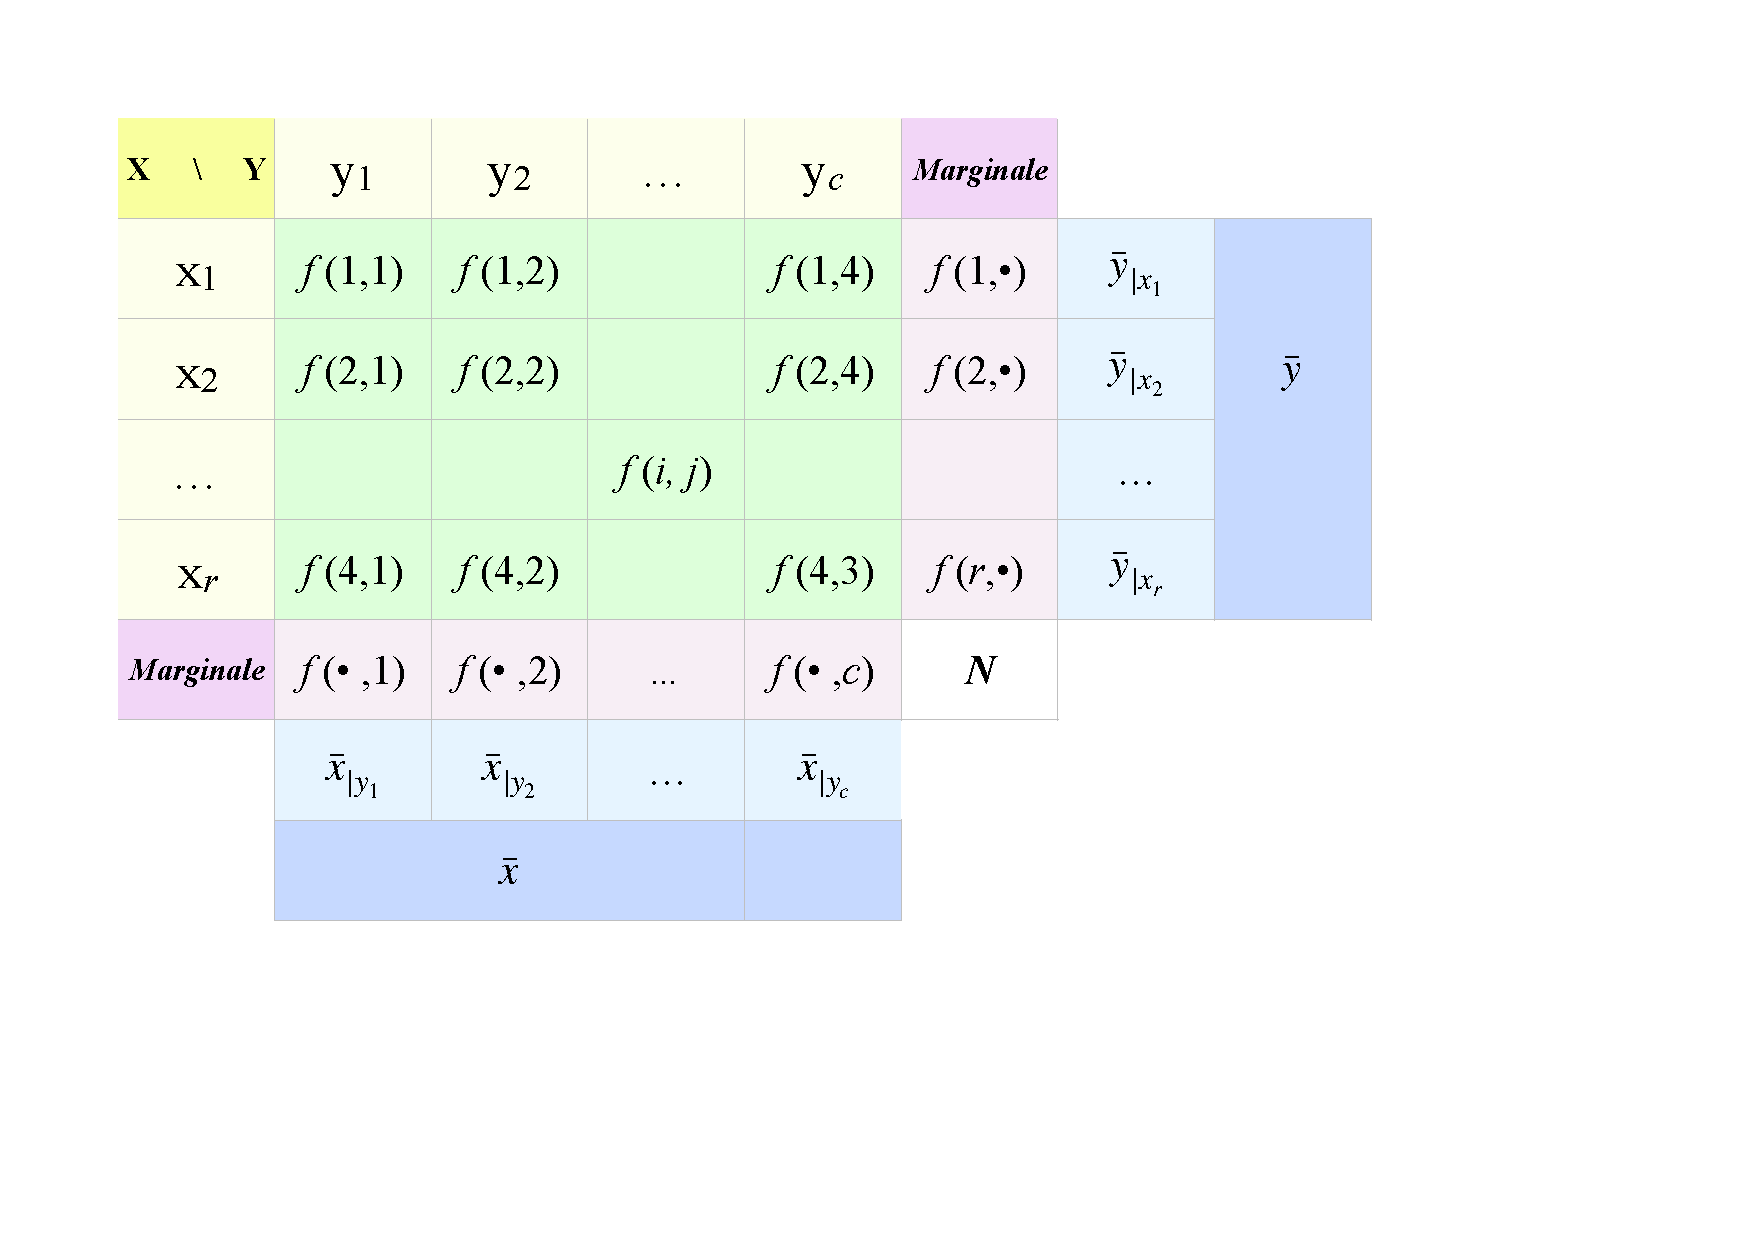
\includegraphics[scale=0.35]{image/tabella.pdf}
                      \end{center}
     \end{definition}
     
       
         \begin{definition}{Frequenza assoluta marginale} permettono di guardare la tabella  
         come una distribuzione di frequenza univariata. 
         
                    \begin{itemize}
                        \item Frequenza assoluta marginale di colonna, $f_{(\bullet ,j)} = \sum_{i=1}^{r} f_{(i,j)}$ 
                      \item Frequenza assoluta marginale di riga, $f_{(i,\bullet)} = \sum_{j=1}^{c} f_{(i,j)}$ 
                    \end{itemize}
                \end{definition}
                
             \begin{definition}{\textbf{Frequenze Condizionate}}  
                La distribuzione condizionata di $X$ rispetto $Y$: 
                    \begin{center}
                        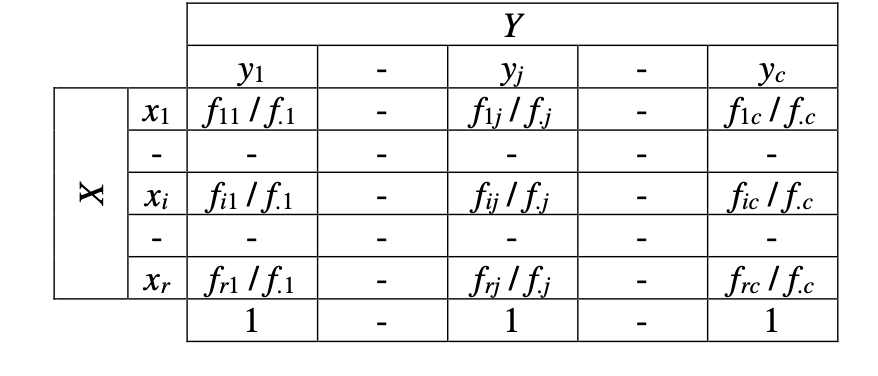
\includegraphics[scale=0.2]{image/fcY.png}
                        \end{center}
                La distribuzione condizionata di $Y$ rispetto $X$:    
                         \begin{center}
                             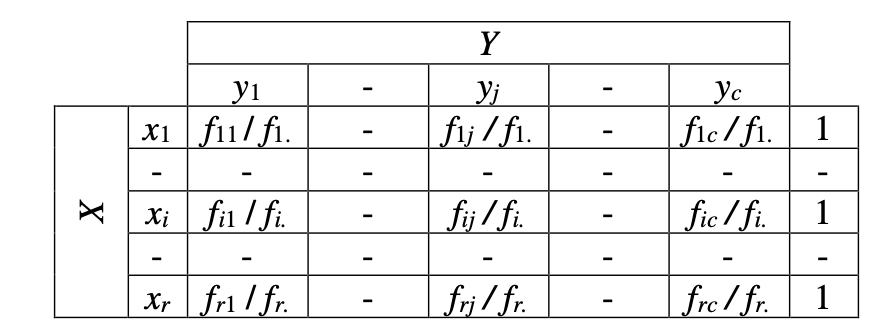
\includegraphics[scale=0.2]{image/fcX.png}
                        \end{center}
                  \end{definition}
    
     \subsection{Analisi statistica bivariata}
        L'analisi statistica bivariata consiste nello stabilire se esiste una qualche \textbf{relazione} tra i due fenomeni considerati.
       
        Il \textbf{metodo per stabilire se sono statisticamente indipendenti} consiste nel confrontare le frequenze condizionate. Se al variare delle modalità del fenomeno condizionante le distribuzioni condizionate non variano, allora i due fenomeni sono statisticamente indipendenti.
        
        La dipendenza si studia sia per caratteri quantitativi sia qualitativi perchè studiamo le frequenze. 
            \begin{itemize}
                \item \textit{Se non esiste alcuna relazione si dirà che X ed Y sono statisticamente indipendenti.}
                \item \textit{  Se due fenomeni non sono statisticamente indipendenti allora esiste una relazione e si dirà che i fenomeni sono connessi.}
            \end{itemize}{}
            
         Se \textbf{esiste una relazione} si procede con delle analisi. 
          \begin{definition}{Contingenze} calcolate per misurare il grado di connessione tra due   modalità
                $$C_{ij}=f_{i,j}-f^*_{i,j}$$
                 dove $f^*_{i,j} = \frac{f_{(i,\bullet)}f_{(\bullet,j)}}{N}$ sono le \textit{\textbf{frequenze teoriche}} che si avrebbero nel caso ci fosse \textit{indipendenza statistica}. 
            \end{definition}
        
         
            \begin{itemize}
                \item $C_{ij} > 0 \implies$  c'è \textbf{\textit{attrazione}}, la connessione è alta. 
                \item $C_{ij} < 0 \implies$ c'è \textbf{\textit{repulsione}}, la connessione è alta. 
                \item $C_{ij} \simeq 0 \implies$ la connessione è bassa. 
            \end{itemize}{}
        
            \begin{definition}{Chi quadro di Pearson}
                    $$ \chi^2 = \sum_{i=1}^{r} \sum_{j=1}^{c}\frac{(f_{ij}-f^*_{ij})^2}{f^*_{ij}} \in [0,N min\{(r-1);(c-1)\}]$$
            \end{definition}
            di conseguenza l'indice normalizzato 
                $$\chi^2_{NORM} = \frac{\chi^2}{\chi^2_{MAX}}=\frac{\chi^2}{N min\{(r-1);(c-1)\}} \in [0,1] $$
        
       \paragraph{}
       
        Se \textbf{almeno} uno dei due fenomeni è \textbf{quantitativo} ad esempio Y, ci si può chiedere se \textbf{\textit{Y dipende in media da X}}, ovvero se al cambiare delle modalità di X cambiano le medie di Y.
         \begin{definition}{Indipendenza in media} Si dice che c'è indipendenza in media se tutte le medie condizionate sono tra loro uguali e quindi uguali alla media marginale:
            $$ \bar{y}|x_1=  \bar{y}|x_2= ... = \bar{y}|x_r= \bar{y}$$
            quindi se fisso una $i^*$ la media di y condizionata ad $x_i$ è uguale a: 
            $$ \bar{y}|x_{i^*}=\frac{\sum_{j=1}^{c}y_jf_{(i^*,j)}}{f_{(i^*,\bullet)}}$$
            $$ \bar{y}= \frac{\sum_{i=1}^{r}\bar{y}|x_if_{(i,\bullet)}}{N}$$
            
        \end{definition}
                    
        
        \paragraph{Indipendenza in media}
        \begin{definition}{Eta Quadro}
        Il modo per misurare la dipendenza in media è data da questa formula
                $$ \eta^2_{Y|X}= \frac {\sigma^2_B}{\sigma^2_Y} =
                \frac{\frac{1}{N}\sum_{i=1}^{r}(\bar{y}|x_i - \bar{y})f_{(i,\bullet)}}
                {\frac{1}{N}\sum_{j=1}^{c}(y_j^2f_{(\bullet,j)} - \bar{y}^2)} \in [0,1] $$
        \end{definition}
        
        \begin{teorema}Se Y dipende in media da X implica che Y è dipendente statisticamente da
            $$
            \eta^2_{Y|X} \implies \chi^2 > 0 $$
        
        \end{teorema}
         \begin{teorema}
          L’indipendenza in media di Y da X non implica l’indipendenza in media di X da Y
        
        \end{teorema}
        
        \subsection{Correlazione lineare}
        Se \textbf{entrambi} i fenomeni sono \textbf{quantitativi} è possibile andare oltre all’analisi dell’indipendenza in media.
        
        \begin{definition}{Covarianza} è una misura di variabilità congiunta definita come 
            \begin{itemize}
               \item $\sigma_{xy} = \sigma_{yx}$
                \item  Quando è nota la distribuzione di frequenza doppia
                $$ \sigma_{xy}  =  \frac{1}{N}\sum_{i=1}^{r}\sum_{i=1}^{c}(x_i-\bar{x})(y_j-\bar{y})f_{ij}$$
                Alternativamente si può calcolare
                $$\sigma_{xy}= \mu_{xy} - \bar{x}\, \bar{y}$$  dove $\mu_{xy}$ è detta media bivariata o media dei prodotti, definita come: 
          $$ \mu_{xy} = \frac{1}{N}\sum_{i=1}^r \sum_{j=1}^c x_i \,y_i \,\,f_{ij}$$
             
             \item Quando ho la matrice di dati grezzi
                 $$ \sigma_{xy} = \frac{1}{n}\sum_{i=1}^{n}(x_i-\bar{x})(y_i-\bar{y})$$
                
            \item Nota che $$\sigma_{xx}                     
                        =\frac{1}{n}\sum_{i=1}^{n}(x_i-\bar{x})(x_i-\bar{x})= \frac{1}{n}\sum_{i=1}^{n}(x_i-\bar{x})^2 = \sigma^2_x$$
                
            \end{itemize}{}
            
          
            Se $(x_i - \bar{x})(y_i -\bar{y})$ sono discordi in segno allora peseranno negativamente sulla somma rendendo piccola la covarianza ed al contrario se sono concordi aumenteranno il valore della covarianza. 
            
            Quindi due serie di dati sono \textbf{statisticamente incorrelate} se $\sigma_{xy}=0$ e viceversa. 
        \end{definition}{}
        
        \begin{teorema}{}
            Statisticamente indipendenti $\implies$ Statisticamente incorrelati
        \end{teorema}

        \begin{definition}{}L'indice di correlazione è definito come 
            $$\rho = \frac{\sigma_{xy}}{\sqrt{\sigma^2_x\sigma^2_y}}$$ 
                \begin{itemize}
                    \item Normalizza la covarianza, perché divide $\sigma_{xy}$ per la radice di $\sigma^2_x \sigma^2_y$
                    \item Senza unità di misura, quindi è confrontabile
                    \item $\rho \in [-1,1]$ e dà indicazioni circa il verso e l'intensità della correlazione
                    \item Se uguale ad $\pm 1$ allora i fenomeni sono perfettamente allineati lungo una retta, il cui coefficiente angolare è $>0$ se $\rho >0$ e viceversa. 
                    \item Se uguale a 0 allora sono incorrelati. 
                \end{itemize}
        \end{definition}
        \paragraph{}
        
         \paragraph{Matrici di Covarianza e Correlazione} 
         \begin{itemize}
             \item Caso bidimensionale $$C = \left[
             \begin{matrix}
                \sigma^2_x &\sigma_{xy} \\
                \sigma_{yx}& \sigma^2_y
             \end{matrix}
             \right]$$
             dove $\sigma_{xy} = \sigma_{yx}$
             
        $$Corr = \left[
             \begin{matrix}
                \frac{\sigma_{xx}}{\sigma^2_x}&\frac{\sigma_{xy}}{\sqrt{\sigma^2_x\,\sigma^2_y}}\\
                \frac{\sigma_{yx}}{\sqrt{\sigma^2_x\,\sigma^2_y}}& \frac{\sigma_{yy}}{\sigma^2_y}
             \end{matrix}
             \right]
             = 
                 \left[ 
                 \begin{matrix}
             \frac{\sigma^2_{x}}{\sigma^2_x}    &\frac{\sigma_{xy}}{\sqrt{\sigma^2_x\,\sigma^2_y}}\\
            \frac{\sigma_{yx}}{\sqrt{\sigma^2_x\,\sigma^2_y}}& \frac{\sigma^2_{y}}{\sigma^2_y}
                 \end{matrix}
                \right]
                =   \left[ 
                 \begin{matrix}
                 1 & \frac{\sigma_{xy}}{\sigma_x\,\sigma_y}\\
                  \frac{\sigma_{yx}}{\sigma_x\,\sigma_y}&1
                  \end{matrix}
                \right]
                = \left[ 
                 \begin{matrix}
                  1 & \rho\\
                  \rho &1
                  \end{matrix}
                \right]
                         $$ 
                \item Caso m variabili 
                $$C = \left[
             \begin{matrix}
                \sigma^2_{x_1}     &\sigma_{x_1x_2}  &...&\sigma_{x_1x_m}\\
                \sigma_{x_1x_2}  & \sigma^2_{x_2}    &...&\sigma_{x_2x_m}\\
                    ...          &             ... &...&          ...   \\
                \sigma_{x_1x_m}  & ...             & ...&\sigma^2_{x_m}
             \end{matrix} 
             \right]\,\,\,
              Corr = \left[
             \begin{matrix}
                1     &\rho_{x_1x_2}  &...&  \rho_{x_1x_m}\\
                \rho_{x_1x_2}  & 1    &...&  \rho_{x_2x_m}\\
                    ...        &  ... &...&         ...   \\
                \rho_{x_1x_m}  & ...  & ...&1
             \end{matrix} 
             \right]$$
             
         \end{itemize} 
       \paragraph{}
        \begin{definition}
          In generale di dice \textbf{momento k-esimo} rispetto a y
            $$M_{k,y} = \frac{1}{n} \sum_{i=1}^n(x_i-y)^k$$
            \begin{itemize}
                \item \textbf{Media} momento primo rispetto all'origine 0$$M_{1,0} = \frac{1}{n} \sum_{i=1}^n(x_i)$$
                \item \textbf{Varianza} momento secondo rispetto alla media $\bar{x}$
                  $$M_{2,\bar{x}} = \frac{1}{n} \sum_{i=1}^n(x_i-\bar{x})^2$$
            \end{itemize}{}
            \end{definition}
        \newpage
        \subsection{Modello di regressione lineare}
        Spesso dato un insieme E di coppie di dati
        $E = \{(x_1,y_1),(x_2,y_2),...,(x_n,y_n)\}$ ci si chiede se esiste una relazione di tipo funzionale tra x e y che descriva soddisfacentemente il legame tra di essi. 
        In tal caso si parla di \textbf{analisi di regressione}, che affronta il problema pensando ad uno dei due caratteri come ad una variabile indipendente, ad esempio $x$, e cerca di stabilire quale funzione $f \in C^k$, all'interno di una specifica classe, consente di scrivere al \textbf{\textit{meglio}} il legame $$y=f(x)$$ Dove y è detta variabile dipendente. \\
        Occorre quindi capire che per \textbf{\textit{meglio}} si intende solitamente la funzione $f$ che \textbf{minimizza le distanze} tra i valori osservati del carattere y e quelli che si otterrebbero per il carattere y se la relazione fosse proprio quella descritta da $f(x)$.
         \bigbreak %per aggiungere spazio tra le linee
        Bisogna trovare la $f$ che minimizzi questa quantità:
        \begin{equation}\label{eq.1}
            g(f) = \sum_{i=1}^n\left[ f(x_i)-y_i\right]^2
        \end{equation}{}
      
        Se si limita l'insieme delle funzioni all'insieme di quelle lineari allora si parlerà di \textbf{regressione lineare}. 
        \paragraph{Regressione Lineare} Riformulando l'equazione (\ref{eq.1}) con vincolo di avere $$f(x) = mx + q\\$$ 
         \begin{equation}\label{eq.2}
            g(m,q) = \sum_{i=1}^n\left[ mx_i+q -y_i\right]^2
        \end{equation}{}
        Il problema si riduce alla determinazione dei coefficienti m e q della retta per cui risulti minima (\ref{eq.2}).
       
        \begin{teorema} Sia $f(x) = mx+q$ la funzione utilizzata nel modello di regressione lineare atta a minimizzare la seguente quantità $$g(m,q) = \sum_{i=1}^n\left[ mx_i+q -y_i\right]^2  \implies m=\frac{\sigma_{xy}}{\sigma^2_x} \,\,;\,\, q=(\bar{y}- \frac{\sigma_{xy}}{\sigma^2_x}\bar{x})$$
        Dove m e q sono i coefficienti che rendono minima la somma dei quadrati, e la retta ottenuta con quei coefficienti è detta \textbf{di regressione lineare}.
       \newpage
         \begin{dimostrazione}
         $$\sum_{i=1}^n\left[ mx_i+q -y_i\right]^2$$ chiamo 
         $\phi(m,q) = \sum_{i=1}^n\left[ mx_i+q -y_i\right]^2$ se voglio che la differenza sia minima devo imporre che le derivate parziali di $\phi(m,q)$ siano uguali a zero.
         $$
             \begin{cases}
                 \frac{\partial\phi(m,q)}{\partial m}=0\\
                  \frac{\partial\phi(m,q)}{\partial q}=0
            \end{cases}
            =  \begin{cases}
                 \partial\frac{\sum_{i=1}^n\left[ mx_i+q -y_i\right]^2}{\partial m}=0\\
                 \partial\frac{\sum_{i=1}^n\left[ mx_i+q -y_i\right]^2}{\partial q}=0
            \end{cases}
             $$
             $$
             =
             \begin{cases}
                 \frac{\sum_{i=1}^n\partial \left[ mx_i+q -y_i\right]^2}{\partial m}=0\\
                 \frac{\sum_{i=1}^n\partial\left[ mx_i+q -y_i\right]^2}{\partial q}=0
             \end{cases}
             = \begin{cases}
                 \frac{\sum_{i=1}^n\partial \left[ y_i - mx_i-q \right]^2}{\partial m}=0\\
                 \frac{\sum_{i=1}^n\partial\left[ y_i - mx_i-q\right]^2}{\partial q}=0
             \end{cases}
             $$
             Risolviamo il primo termine del sistema: 
             $$\frac{\partial\phi(m,q)}{\partial m} = \sum_{i=1}^{n} [2(y_i-mx_i-q)(-x_i)] =  -2\sum_{i=1}^{n} [(y_i-mx_i-q)(x_i)]=0 $$ 
             $$\implies\sum_{i=1}^{n} [(y_i-mx_i-q)(x_i)]=0 
             $$
             
              Risolviamo il secondo termine del sistema: 
             $$\frac{\partial\phi(m,q)}{\partial m} = \sum_{i=1}^{n} [2(y_i-mx_i-q)(-1)] =  -2\sum_{i=1}^{n} [(y_i-mx_i-q)]=0 $$ 
             $$\implies\sum_{i=1}^{n} [(y_i-mx_i-q)]=0 
             $$
             Quindi il sistema: 
             $$
              \begin{cases}
               \sum_{i=1}^{n} [(y_i-mx_i-q)(x_i)]=0 \\
               \sum_{i=1}^{n} [y_i-(mx_i+q)]=0 
             \end{cases}
             $$
             Ricavo q dalla seconda: 
             $$\sum_{i=1}^{n}y_i-\sum_{i=1}^{n}mx_i+\sum_{i=1}^{n}q=
             \sum_{i=1}^{n}y_i-m\sum_{i=1}^{n}x_i-nq=0$$
             $$
                nq = \sum_{i=1}^{n}y_i-m\sum_{i=1}^{n}x_i
             $$
             $$ q = \frac{1}{n}\sum_{i=1}^{n}y_i-\frac{m}{n}\sum_{i=1}^{n}x_i$$
             $$ q =\bar{y}-m\bar{x}$$
             Sostituisco q nella prima: 
             $$
             \begin{cases}
               \sum_{i=1}^{n} [(y_i-mx_i-\bar{y}+m\bar{x})(x_i)]=0 \\
               q =\bar{y}-m\bar{x}
             \end{cases}
             $$
             Riscrivo la prima equazione: 
             $$\sum_{i=1}^{n} [(y_i-mx_i-\bar{y}+m\bar{x})(x_i)]=
               \sum_{i=1}^{n} [((y_i-\bar{y})+(m\bar{x}-mx_i))(x_i)]=$$
               $$\sum_{i=1}^{n} [((y_i-\bar{y})-m(x_i-\bar{x}))(x_i)]= 
                 \sum_{i=1}^{n} (y_i-\bar{y})(x_i) -m\sum_{i=1}^{n}(x_i-\bar{x})(x_i) =0
               $$
               $$m \sum_{i=1}^{n}(x_i-\bar{x})(x_i)= \sum_{i=1}^{n} (y_i-\bar{y})(x_i)$$
               $$m =    \frac{\sum_{i=1}^{n} (y_i-\bar{y})(x_i)}{\sum_{i=1}^{n}(x_i-\bar{x})(x_i)} =  \frac{\sum_{i=1}^{n} (x_i-\bar{x})(y_i-\bar{y})}
                    {\sum_{i=1}^{n}(x_i-\bar{x})^2} $$
                    
                $$
                        m= \frac{\sigma_{xy}}{ \sigma^2_x}\,\,;\,\, q = \bar{y} - \frac{\sigma_{xy}}{ \sigma^2_x}\bar{x}
                $$
                    
            Dove il numeratore:
            $$\sum_{i=1}^{n} (x_i-\bar{x})(y_i-\bar{y}) =  \sum_{i=1}^{n}x_i(y_i-\bar{y}) - \sum_{i=1}^{n}\bar{x}(y_i-\bar{y})$$
            $$
                = \sum_{i=1}^{n}x_i(y_i-\bar{y})- \bar{x}\sum_{i=1}^{n}(y_i-\bar{y})
                = \sum_{i=1}^{n}x_i(y_i-\bar{y})
            $$
               
            Dove il denominatore:
               $$ \sum_{i=1}^{n}(x_i-\bar{x})^2  = \sum_{i=1}^{n}(x_i-\bar{x})(x_i-\bar{x})
                = \sum_{i=1}^{n}x_i(x_i-\bar{x})- \sum_{i=1}^{n}\bar{x}(x_i-\bar{x})
               $$
               $$
                   = \sum_{i=1}^{n}x_i(x_i-\bar{x})-\bar{x}\sum_{i=1}^{n}(x_i-\bar{x})= 
                    \sum_{i=1}^{n}x_i(x_i-\bar{x})
               $$
               
         \end{dimostrazione}
        \end{teorema}
        \newpage
        
        \paragraph{Adattamento della retta ai dati} Per misurare il grado di adattamento della retta di regressione lineare ai dati si utilizza la scomposizione della varianza applicata alla retta. 
               \begin{center}
                             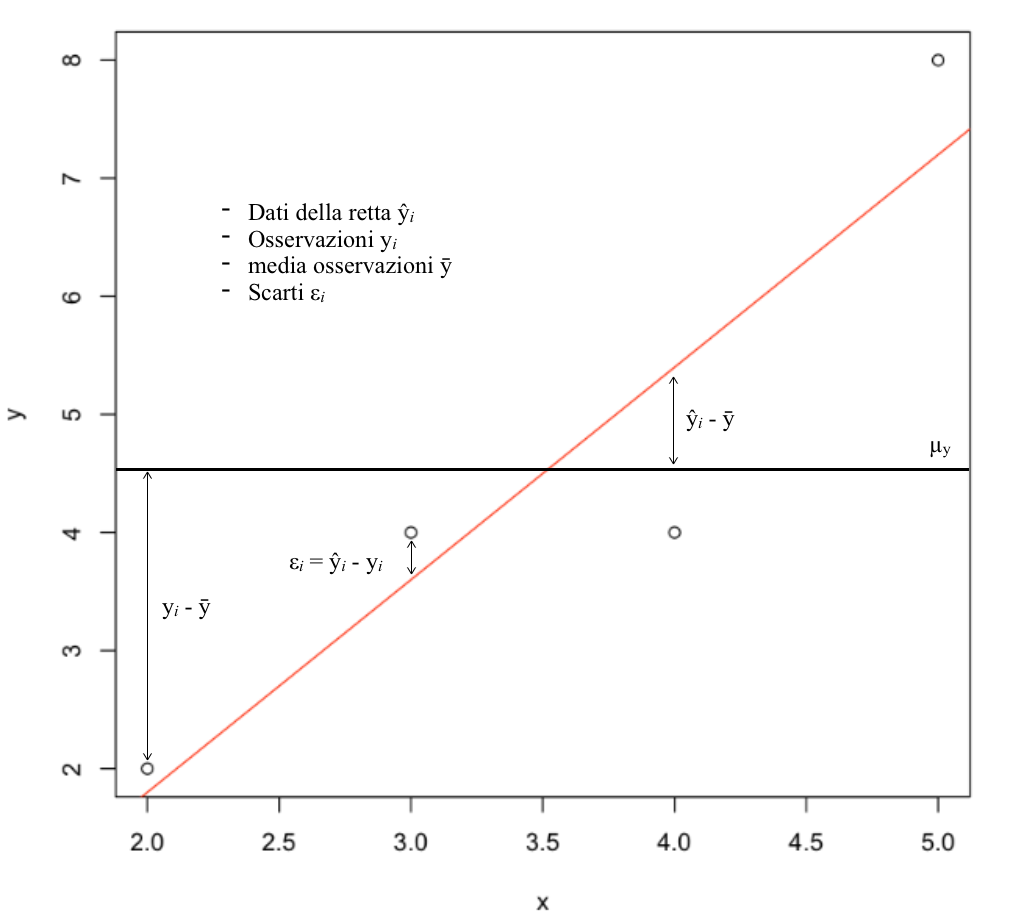
\includegraphics[scale=0.33]{image/regressione.png}
                \end{center}
           
          \begin{teorema}{} La scomposizione della varianza della retta di regressione lineare 
          $$ \sigma^2_y= \sum_{i=1}^n(y_i-\bar{y})^2= 
          \sum_{i=1}^n(y_i-\hat{y_i})^2. +  \sum_{i=1}^n(\hat{y_i}-\bar{y})^2 $$
          
          Ossia la varianza totale è uguale alla varianza spiegata più quella residua. 
          
          \begin{dimostrazione}
          
          \end{dimostrazione}
           $$ \sigma^2_y= \sum_{i=1}^n(y_i-\bar{y})^2= 
              \sum_{i=1}^n((y_i-\hat{y_i})+(\hat{y_i}-\bar{y}))^2$$
           $$
             = \sum_{i=1}^n((y_i-\hat{y_i})^2+(\hat{y_i}-\bar{y})^2+2(y_i-\hat{y_i})(\hat{y_i}-\bar{y}))=
           $$
           
           $$
                 = \sum_{i=1}^n(y_i-\hat{y_i})^2+ \sum_{i=1}^n(\hat{y_i}-\bar{y})^2+\sum_{i=1}^n2(y_i-\hat{y_i})(\hat{y_i}-\bar{y})
           $$
           Analizziamo l'ultimo termine: 
           $$
                \sum_{i=1}^n2(y_i-\hat{y_i})(\hat{y_i}-\bar{y})
           $$
           Noi sappiamo che $\hat{y_i}=f(x)=mx_i+q=$ e $\bar{y}= m\bar{x}+q$
           $$
            \implies (\hat{y_i}-\bar{y})= mx_i+q -m\bar{x}-q = m(x_i-\bar{x})
           $$
           Quindi: 
           $$
               \sum_{i=1}^n(y_i-\hat{y_i})^2+ \sum_{i=1}^n(\hat{y_i}-\bar{y})^2+\sum_{i=1}^n2(y_i-\hat{y_i})m(x_i-\bar{x})
           $$
           Ma la somma degli scarti di $x_i$ dalla media è uguale a zero di conseguenza: 
           $$
                 \sigma^2_y= \sum_{i=1}^n(y_i-\bar{y})^2=  \sum_{i=1}^n(y_i-\hat{y_i})^2+ \sum_{i=1}^n(\hat{y_i}-\bar{y})^2
           $$
          \end{teorema}
            
         \paragraph{L'indice di adattamento della retta}
         $$ \rho^2 = \frac{var(retta)}{\sigma^2_y}=  
         \frac{\sum_{i=1}^n(y_i-\hat{y_i})^2}
              {\sum_{i=1}^n(y_i-\hat{y_i})^2+ \sum_{i=1}^n(\hat{y_i}-\bar{y})^2}
         $$
         
         \newpage
         \section{Probabilità}
         La probabilità è una disciplina di carattere matematico che permette di affrontare l’analisi delle situazioni che hanno un esito imprevedibile a priori e pertanto con conseguenze incerte.
         
         È quindi una teoria (assiomatica o frequentista o soggettiva) che riguarda il calcolo della probabilità del verificarsi di certi eventi composti di eventi elementari strumento di base per la
         
         Esistono diverse definizioni di probabilità anche se ad oggi non esiste una universale. 
         \begin{itemize}
             \item Classica
             \item Frequentista
             \item Soggettivista 
             \item Assiomatica, quella presentata. 
         \end{itemize}{}
         
         \subsection{Impostazione assiomatica}
         
         \begin{definition}{}
             Sia $\Omega$ un insieme di diversi possibili esisti, ben distinti tra di loro. Ogni sottoinsieme  $A\subset \Omega$ viene detto \textbf{evento}. \\
         \end{definition}
         
         \begin{definition}{}
            $\forall A_i \subset \Omega$ è associata una quantità numerica detta $P(A)$ il cui significato varia dall'impostazione
         \end{definition}
         
         Un passo fondamentale per superare le interpretazione sul concetto di probabilità fu fatto da Kolmogorov nel 1933.
         
          \begin{definition}{} 
          Sia $\Omega$ un insieme finito o infinito di elementi esso viene detto \textbf{spazio campione} o \textbf{spazio campionario}.\\
          Ogni sottoinsieme $A$ di $\Omega$ viene detto \textbf{evento} e può essere: 
         
          \begin{itemize}
              \item Elementare se costituito da un singolo elemento di $\Omega$
              \item Composto se costituito da più di un elemento di $\Omega$
          \end{itemize}{}
          
          \end{definition}
         
            \begin{definition}{} 
                Si definisce insieme delle parti di $\Omega$, l'insieme di tutti i suoi sottoinsiemi e lo si denota tramite $$\wp(\Omega)$$
                La probabilità deve essere definita per tutti gli elementi di $\wp(\Omega)$ con particolari proprietà. 
            \end{definition}{} 
            
            \begin{definition}{} 
                Siano  $A, B$  eventi $\subset \Omega$ sono incompatibili se sono disgiunti. \\
                $$ A \cap B = \emptyset$$
            \end{definition}{} 
            
             \begin{definition}{}
             Secondo Kolmogorov viene detta \textbf{misura di probabilità} ogni applicazione
             $$P\colon \wp(\Omega)\mapsto \mathbb{R}^+_0$$
             che associa un numero reale ad ogni sottoinsieme di $\Omega$ in cui valgono le seguenti \textbf{proprietà}:
             \begin{itemize}
                 \item Per ogni $A\subset \Omega\,\, P(A)\geq0$. Interpretando P(A) come frequenza relativa allora essa è compresa tra [0,1]
                 \item $P(\Omega) = 1$. È certo che si realizzi uno qualsiasi evento tra tutto quelli di $\Omega$. 
                 \item Dato $F=\{A_i, i \in I \subset N \}$ insieme di eventi incompatibili allora vale che
                 $$ P\left(\bigcup_{i\in I} A_i\right) = \sum_{i\in I} P(A_i)$$ 
             \end{itemize}{}
             Ogni misura di probabilità assegna valori numerici a sottoinsiemi di $\Omega$ e non ai suoi elementi, quindi ad eventi elementari. 
            \end{definition}{} 
            
            Ne segue dalle proprietà sopra elencate che: 
            \begin{itemize}
                \item $\forall A \subseteq \Omega\,\, P(\bar{A}) = 1 - P(A)$
                \item $\forall  A \subseteq \Omega\,\, P(A)\leq 1$
                \item $ \forall A,B \subseteq \Omega\,\,, A \subseteq B\,\,$ allora $P(A)\leq P(B) $
                \item $\forall A,B \subseteq \Omega$ vale 
                $$P(A\cup B)=P(A)+P(B) - P(A\cap B)$$
            \end{itemize}{}
            
            \begin{dimostrazione}{}
                 $P(\bar{A}) = 1 - P(A)$
                
                 $$  1 = P(\bar{A}\cup A)= P(\bar{A})+P(A) - P(\bar{A}\cap A)= P(\bar{A})+P(A) 
                 $$
            \end{dimostrazione}
             \bigbreak
             
             \begin{definition}{}
             Siano A e B due eventi qualsiasi dello spazio campionario e sia P(A) $\neq$ 0, 
             la probabilità che si verifichi l'evento B dato l'evento A si dice \textbf{probabilità condizionata} di B dato A definita come
             $$P(B|A) = \frac{P(A\cap B)}{P(A)}$$
             di conseguenza vale che: 
             $$P(B|A) P(A) = P(A\cap B)$$
             \end{definition}{} 
             
             \begin{definition}{}
             Due eventi si dicono indipendenti se $$P(B|A) = P(B) $$
             Quindi la $P(A\cap B)= P(B|A)P(A)=P(B)P(A)$
             \end{definition}{} 
             
             
             \begin{teorema}{}
                Siano $B_1\,\,\,B_2$ eventi incompatibili e $B_1 \cup B_2 = \Omega$ e $A \subset \Omega$
                $$\implies$$ 
                $ A\cap B_1 $ e   $ A\cap B_2 $ sono anch'essi disgiunti. 
                \begin{center}
                             \includegraphics[scale=0.33]{image/probabilità.png}
                \end{center}
                
                Quindi: 
                $$
                     P(A) = P(A\cap B_1) +P(A\cap B_2) = P(B_1)P(A|B_1) +P(B_2)P(A|B_2)
                $$
                
                %COROLLARIO ESTESO SU PIU INSIEMI
            \end{teorema}
             
             
             \begin{teorema}{} %Mettere  il teorema di BAYES
             
              \end{teorema}
              \newpage
              \subsection{Variabili Casuali}
             
              \subsubsection{Unidimensionali}
                
                \begin{definition}{}
                Una variabile casuale è una applicazione definita come
                
                $$  
                    X\colon \Omega \mapsto \mathbb{R} 
                $$
                tale per cui  $\forall \, \omega \in \Omega$ si associ un numero $\mathbb{R}$\\
                
                $X(\Omega)$ o supporto può essere:%X(\wp(\Omega))
                 \begin{itemize}
                    \item \textbf{Discreto}, associa ad ogni elemento di $ \Omega$ un numero finito di valori o un'infinità numerabile
                    \item \textbf{Continuo}, associa ad ogni elemento di $ \Omega$ un'infinità di valori non numerabile
                \end{itemize}
            
                \end{definition}
                
                \paragraph{Concetti variabile casuale}
                 In base alla definizione, quello che interessa di una variabile casuale è calcolare la probabilità che essa assuma certi valori.\\
                 Quindi è possibile assegnare delle probabilità ad eventi del tipo\bigbreak
                 
                 $  ``X\in B \subseteq \mathbb{R}"  $ va pensato come un evento di $\Omega$
                 
                 $$    
                     P(\{ X\in B\}) =P(\{ \omega \in \Omega : X(\omega) \in B\})
                 $$
                 
                 \bigbreak
                
                     \paragraph{Caso discreto}
                     \begin{definition}{} Sia X una variabile casuale discreta e siano $\{x_1 ,x_2 ,...\}$ il supporto. 
                     Si dice funzione di probabilità discreta della v.c X la funzione
                         $$
                            f_X\colon \mathbb{Z} \mapsto [0,1]:  z \longmapsto f_X(z) = P(\{\omega \in \Omega : X(\omega) =z\}) = P(X=z)
                         $$
                          tale che associa ad ogni valore del supporto della variabile aleatoria X la sua probabilità.
                    
                    Proprietà: 
                        \begin{itemize}
                            \item $f(z) \geq 0 \,\,\, \forall z \in \mathbb{Z} $
                        \end{itemize}{}
                  \end{definition}        
                 
                  \begin{definition}{} 
                     Si definisce funzione di ripartizione di una v.c. X la funzione
                     $$
                        F_X(t) \colon \mathbb{R} \mapsto [0,1]
                     $$
                     
                     $$ 
                        t\longmapsto P(X\leq t) = \sum_{k : t_k \leq t} f(t_k)  = F_X(t)
                     $$
                     Dove $x_k\in X(\Omega)$ e $f(x_k)= P(X=x_k)$\\
                     
                     \bigbreak
                     Proprietà: 
                     \begin{itemize}{}
                         \item Monotona crescente
                         \item Il suo codominio è a gradino, (siamo nel caso discreto). 
                        \item Deve valere che
                                $$\lim_{t\mapsto +\infty}  F_X(t)=1 $$  $$\lim_{t\mapsto 0}  F_X(t)=0 $$
                                $$\lim_{t\mapsto t_0^+}  F_X(t_0)=1$$
                         \item $\forall\,\, \alpha \in [0,1] $ si dice quantile di ordine $\alpha$, quel valore $x_{\alpha}$ tale per cui 
                         $$ 
                            F(x_{\alpha}) = \alpha
                         $$
                         \item $\sum_{k=1,2,..} f(x_k) = 1$ estesa a tutti i valori assunti dalla v.c. X
                     \end{itemize}{}
                    
                   \end{definition}  
                 
               
                         
                \paragraph{Caso continuo}
                
                \begin{definition}{} 
                    Si dice variabile aleatoria continua se la corrispondente funzione di ripartizione $F_X(t)$ è continua.
                    In particolare si dice \textbf{assolutamente continua} se esiste una funzione
                    $$
                        f_{X} \colon \mathbb{R} \mapsto \mathbb{R^+}:  t \longmapsto f_X(t)
                    $$
                    tale che verifichi
                    $$
                      F_X(t) =   \int_{-\infty}^{t} f_X(u)du \,\,\,\forall t \in \mathbb{R} 
                    $$
                    
                    dove $f_{X} $ è detta \textbf{densità di probabilità} della v.c X con le seguenti proprietà: 
                        \begin{itemize}
                            \item $f_X(t) \geq 0$
                            \item $\int_{-\infty}^{+\infty} f_X(t)dt =1$
                        \end{itemize}{}
                \end{definition}   
                
                
                
                 \begin{definition}{} Si dice supporto della v.c. X l'insieme 
                 $$S= \{ t \in \mathbb{R}: f_x(t) \neq 0 \}$$
                
                \end{definition}   
                
                \paragraph{Osservazioni}
                \begin{enumerate}
                    \item La probabilità di una v.c. X di assumere un valore preciso$P(X=t_0)=0$
                            \begin{dimostrazione}
                                $$ 
                                    P(X=t_0) = P(x\leq t_0) - \lim_{t->t^-_0}P(X\leq t) =  
                                $$
                                $$
                                    = F_X(t_0) - P(X\leq t_0) = F_X(t_0) -F_X(t_0) = 0
                                $$
                            \end{dimostrazione}
                    
                    \item A tale proposito \textit{(1.)} ha invece senso chiedersi 
                            $$
                                P(X\in(a,b]) = F_X(b)-F_X(a)= \int_{-\infty}^{b} f_X(u)du- \int_{-\infty}^{a} f_X(u)du
                            $$
                            $$
                                \int_a^b  f_X(u)du\,\, , \,\, a<b
                            $$
                    
                    \item Quindi se $\exists F_X(t)$ la sua funzione di densità è definita come: 
                                $$
                                    f_x(t)= \frac{\partial F_X(t)}{\partial t}  
                                $$
                \end{enumerate}{}
                
                
                \subsubsection{Multidimensionali}
                \begin{definition}Si dicono v.c. multidimensionale assolutamente continue, l'applicazione
                $$  
                    (X_1,X_2,...,X_n)\colon \Omega \mapsto \mathbb{R}^n
                $$
                \end{definition}
                \paragraph{Corollario} \textit{Nel caso bidimensionale} $(X,Y)\colon \Omega \mapsto \mathbb{R}^2$
                
                \begin{definition} Siano X,Y due v.c. tale che  $(X,Y)\colon \Omega \mapsto \mathbb{R}^2$
                Allora si dice funzione di ripartizione congiunta: 
                    $$
                        F_{X,Y} \colon \mathbb{R}^2 \mapsto [0,1] \subseteq \mathbb{R}\,\,:\,\,
                        (t,s)\longmapsto P(\{X\leq t\}\cap\{Y\leq s\})
                    $$
                \end{definition}
                
                \begin{definition} Siano X,Y due v.c. tale che  $(X,Y)\colon \Omega \mapsto \mathbb{R}^2$ si dicono assolutamente continue se $\exists$
                    $$
                        f_{XY}(t,s)\colon \mathbb{R}^2 \mapsto  \mathbb{R}^+
                    $$
                    tale che: 
                            $$
                                F_{XY}(t,s) = \int_{-\infty}^{t}\int_{-\infty}^{s} f_{XY}(u,v)dudv \,\, 
                                \forall (t,s) \in \mathbb{R}^2
                            $$
                    
                 \end{definition}
                 
                 
                 \paragraph{Osservazioni}
                \begin{enumerate}
                    \item Data la $F_{XY}(t,s)$ la coppia di v.c X,Y assume valori in un qualsiasi sottoinsieme rettangolare $(a_1,b_1)\times(a_2,b_2)$
                    \item Definiamo la probabilità 
                    $$
                        P((X,Y)\in (a_1,b_1]\times(a_2,b_2]) = \int_{a_1}^{b_1}\int_{a_2}^{b_2} f_{XY}(u,v)dudv
                    $$
                \end{enumerate}
                
                 \begin{definition}Siano X,Y due v.c. tale che  $(X,Y)\colon \Omega \mapsto \mathbb{R}^2$ 
                 si dicono stocasticamente indipendenti   
                    
                 $$
                    \rightleftharpoons
                   \forall (t,s)\in \mathbb{R}^2 \,\,vale\,\, F_{XY}(t,s)=F_X(t)F_Y(s)
                 $$
                 Ne segue che: 
                    $$
                        P(\{X\in A\}\cap \{Y\cap B\}) = P(X\in A) P(Y\in B) \,\, \forall           A,B\subseteq \mathbb{R}
                    $$
                Ed inoltre segue che quando sono assolutamente continue: 
                $$
                    f_{XY}(t,s) = D(F_X(t))*F_Y(s) + D(F_Y(s))*F_X(t) 
                $$
                
                 \end{definition}
                 
                 
                 \subsubsection{Indici di tendenza centrale}
                 Analogamente a quanto visto nel \textit{capitolo 2.1} gli indici di tendenza centrale associate alle variabili aleatorie sono grandezze numeriche in grado di sintetizzare, con un solo valore, le principali caratteristiche delle loro distrubuzioni. 
                 
                 \bigbreak
                 
                 Quindi data una v.c. X unidimensionale con supporto $ S\subseteq  \mathbb{R}$ dove \#S=\textit{n} e $\forall t \in S$ è associata la sua $f_X(t)$
                 
                 \begin{itemize}
                 
                    \item \textbf{Moda}, definita come la quantità $\Tilde{X}\in B$ 
                        \begin{itemize}
                            \item Se X v.c. \textbf{\textit{discreta}}:  
                                che corrisponde al massimo valore della distribuzione di probabilità. 
                            \item Se X v.c. \textbf{\textit{continua}}:
                              che corrisponde al massimo valore della funzione di densità $f_X(t)$.
                        \end{itemize}
                          Potrebbe capitare di avere diversi punti di massimo per le due funzioni, in analogia alla statistica descrittiva, si parlerà di distribuzioni multimodali. 
                            
                     \item \textbf{Valore atteso}, corrispondente alla media dei dati statistici.
                        \begin{itemize}
                            \item Se X v.c. \textbf{\textit{discreta}}:  
                            $$
                                \sum_{i=1}^{n} s_i f_X(s_i)= s_1P(X=s_1)+ s_2P(X=s_1)+...+ s_nP(X=s_n)=
                             $$
                             $$
                                =s_1\frac{\gamma_1}{n}+s_2\frac{\gamma_2}{n}+...+s_n\frac{\gamma_n}{n}=\frac{s_1\gamma_1+s_2\gamma_2+...+s_n\gamma_n}{n}
                             $$
                             Ossia significa trovare il baricentro della nostra distribuzione, ipotizzando che $\frac{\gamma_j}{n} = P(X=s_j)$ siano i pesi.  Quindi fornisce un’indicazione di massima del posizionamento della variabile lungo l’asse dei numeri reali.
                               \begin{center}
                                       \includegraphics[scale=0.33]{image/valore atteso.png}
                               \end{center}
                               
                               \paragraph{Corollario}La media aritmetica è un caso particolare del valore atteso, ossia quando i pesi sono uguali da 1, in altri termini  $\gamma_j = 1\,\, \forall j$
                               $$
                                    E[X]= s_1\frac{\gamma_1}{n}+s_2\frac{\gamma_2}{n}+...+s_n\frac{\gamma_n}{n}= \frac{s_1+s_2+...+s_n}{n}= \frac{1}{n}\sum_i^n s_i = \bar{X}
                                $$
                                
                             \item Se X v.c. \textbf{\textit{continua}}:
                             $$
                                \int_{-\infty}^{+\infty}u\,f_X(u)\,\,du
                             $$
                             
                             \paragraph{Proprietà del valore atteso}
                             \begin{itemize}
                                 \item Se $\forall s_i \in S\,\, s_i=\alpha$ con $P(X=\alpha)=\frac{1}{n} \iff E[X]=\alpha$ 
                                 \begin{dimostrazione}
                                    $E[X]= \sum_{i=1}^ns_iP(X=s_i)=\sum_i^n\alpha\frac{1}{n}$
                                    $=\frac{\alpha}{n}\sum_i^n=\frac{\alpha}{n}n=\alpha$
                                   \bigbreak
                                    In maniera analoga si dimostra ($\implies$)
                                \end{dimostrazione}
                                
                                \item Se $ Y=aX+b \implies E[Y]=E[aX+b]=aE[X]+E[b]=aE[X]+b$
                                
                                \item Sia $y = g(X)$ funzione della variabile casuale $$E[y]=\int_{-\infty}^{+\infty}g(u)f_X(u) du$$
                            
                             \end{itemize}{}
                        \end{itemize}{}
                       
                    \item \textbf{Varianza}, è una misura della dispersione dei valori della variabile casuale X attorno al valor medio.
                    
                     
                 \end{itemize}{}
                 
                 
                 
                 
                 
                 
                 
                 
                 
                 
\end{document} 
